\textbf{Problem 3.}

Let us solve the Poisson equation:
\begin{align*}
    -u_{xx} = f(x), \quad \text{for} \quad x\in(0,1)
\end{align*}

with boundary conditions $u(0)=u(1)=0$, numerically using a 2nd order central difference approximation and a uniform grid of size $\Delta x$.  We wish to study the accuracy of the numerical scheme and the order of convergence of the solution using three different modified norms, $\norm{\cdot}_1^*$, $\norm{\cdot}_2^*$, $\norm{\cdot}_\infty^*$ defined by
\begin{align*}
    \norm{\underline{v}}_P^* = \left( \sum_{i=1}^n \Delta x \abs{v_i}^p \right)^{1/p}
    = \Delta x^{1/p} \norm{\underline{v}}_p
\end{align*}

for the following three functions:

\begin{enumerate}[label=(\alph*),itemsep=0mm]
    
    \item $f(x) = (6x + 2x^2)e^x$
    \item $$f(x) = \begin{cases}
        2 & \text{for} \> 0 \leq x \leq 1/2 \\
        0 & \text{for} \> 1/2 < x \leq 1
    \end{cases}$$
    \item $f(x) = 3x$
    
\end{enumerate}

We first begin by plotting the numerical solutions (scatter plots) against the exact solution (black line) as in Fig. \ref{hw2_qn3_num}.  We start by taking $\Delta x = 1/10$ and then refine it a further 8 times, and we see that as $\Delta x \rightarrow 0$ then the numerical solution converges to the analytic solution.

\begin{figure*}[h!]
\centering
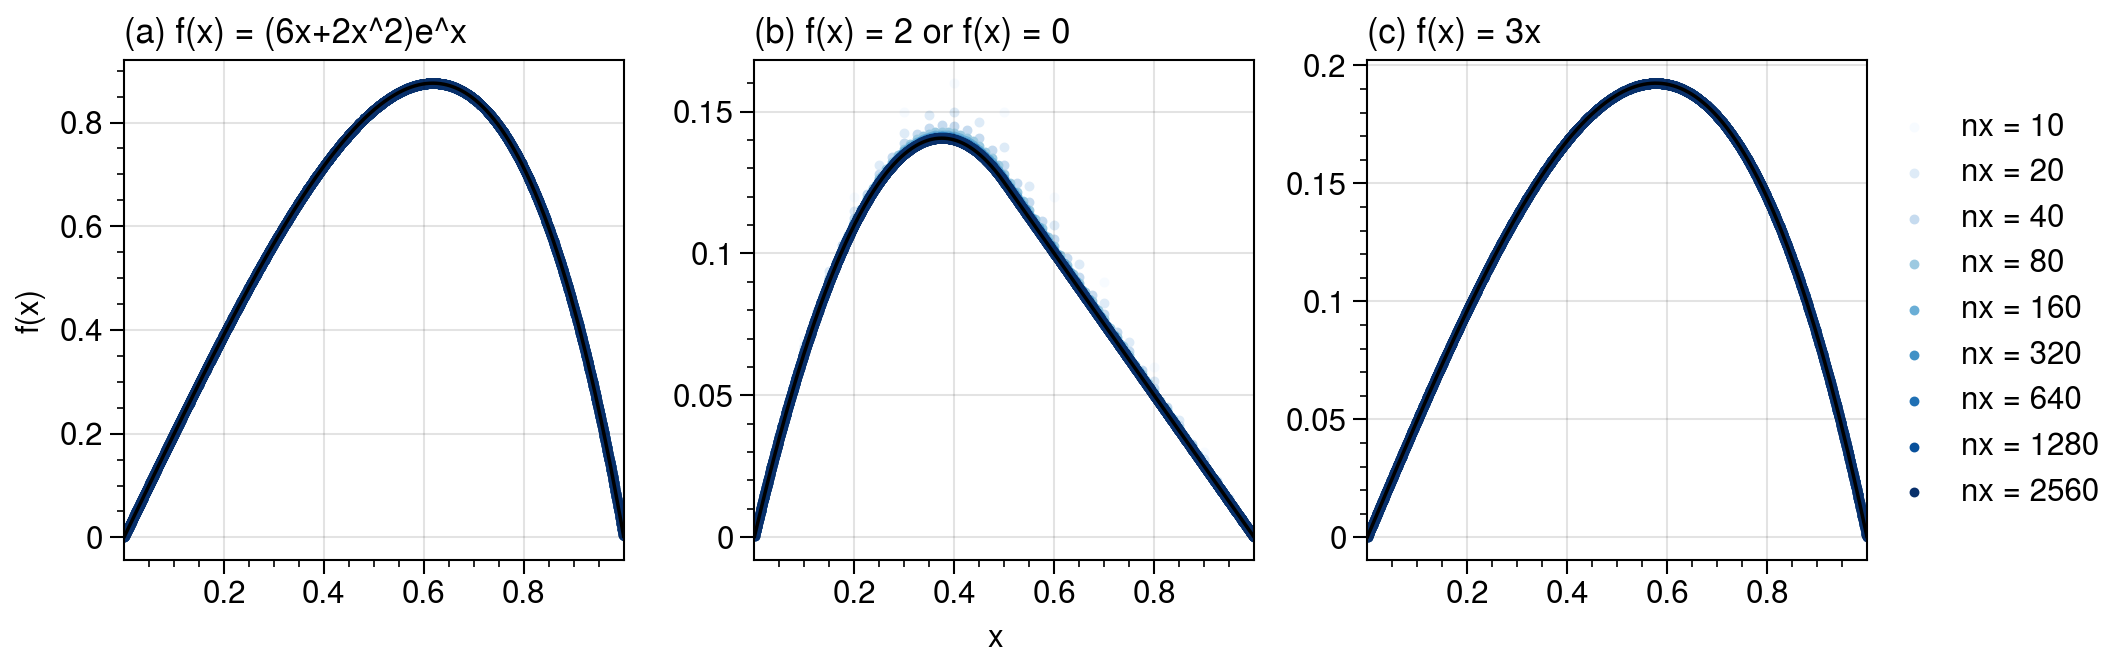
\includegraphics[width=\textwidth]{figures/hw2_qn3_numericalsol.png}\\
\caption{A plot of the numerical solutions against the exact analytical solution (black lines).  The numerical solution for (b) converges more slowly than in (a) and (c), indicating a lower order of convergence, which we corroborate in Fig. \ref{hw2_qn3_pnorm}}
\label{hw2_qn3_num}
\end{figure*}

Now, we calculate the order of convergence by plotting the values of the three different modified norms, $\norm{\cdot}_1^*$, $\norm{\cdot}_2^*$, $\norm{\cdot}_\infty^*$ against $\Delta x$ (Fig. \ref{hw2_qn3_pnorm}).  We see that function (a) has 2nd order of convergence, (b) has first order of convergence, which (c) the solutions are more or less exact and are likely just due to machine precision.

\begin{figure*}[h!]
\centering
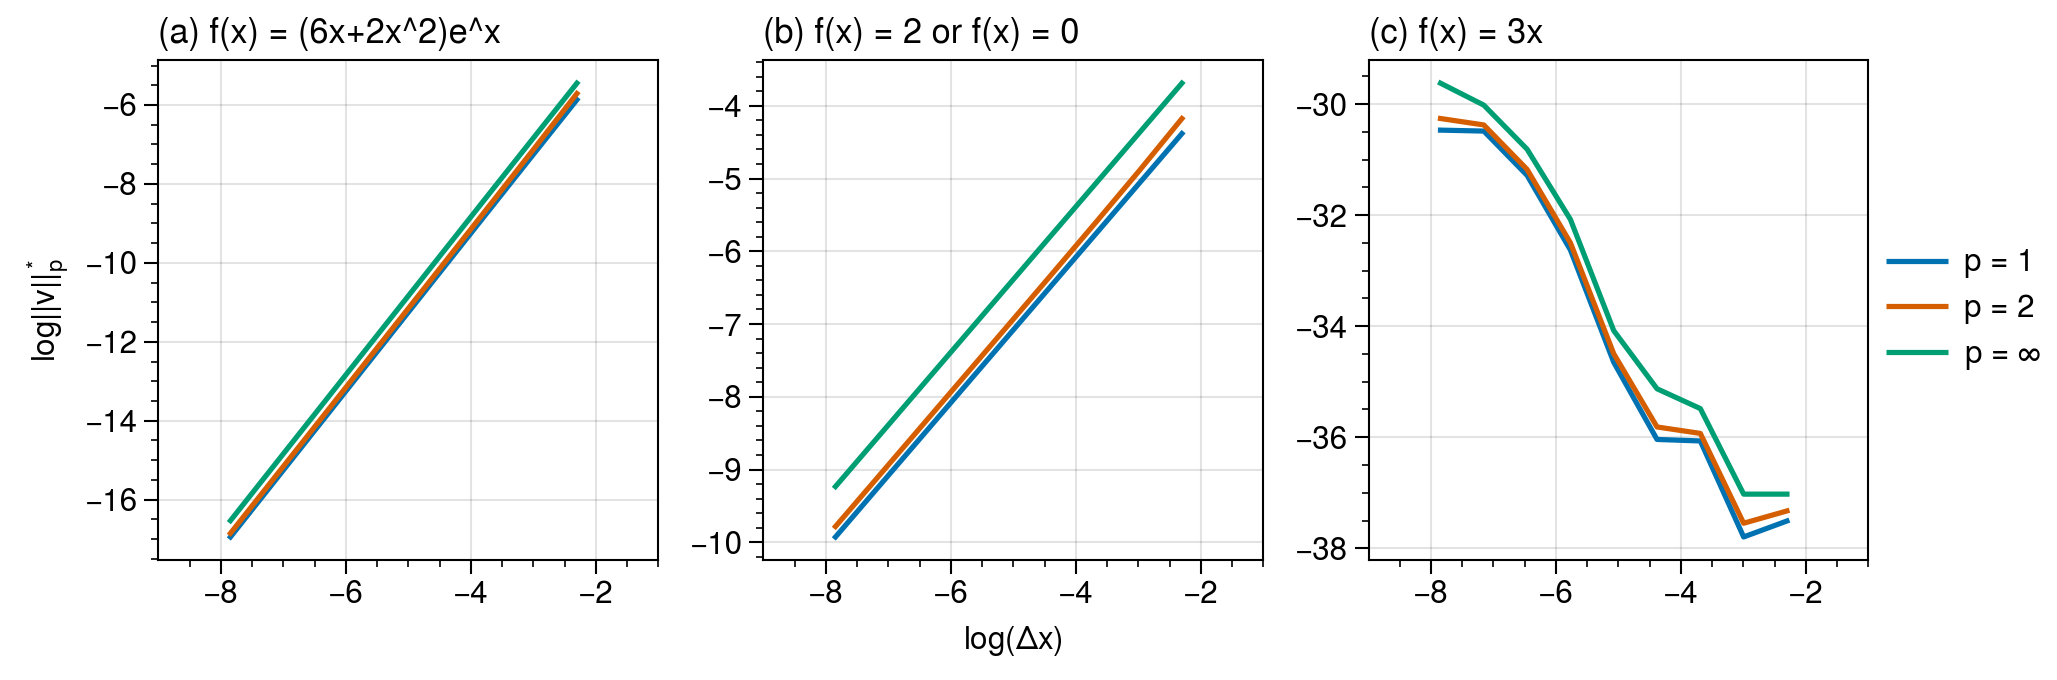
\includegraphics[width=\textwidth]{figures/hw2_qn3_pnorm.png}\\
\caption{A plot of modified $p$-norms against the grid spacing $\Delta x$.}
\label{hw2_qn3_pnorm}
\end{figure*}

Here, we use the modified norms, because, as $\Delta x$ decreases, the number of terms to be summed increases, and therefore this increases the matrix norm explicitly.  Thus, for a direct comparison across matrices with a different number of terms, we must divide the error by the number of terms, which is represented by $\Delta x$.  This will give us the average error that is to be expected for individual points.